\documentclass{article}

%%%%%%%%%%%%%%%%%%%%%%%%%%%%%%%%%%%%%%%%

\usepackage[utf8]{inputenc}

%%%%%%%%%%%%%%%%%%%%%%%%%%%%%%%%%%%%%%%%

\usepackage{tikz}
\usepackage{pgfplots}
\pgfplotsset{compat=1.13}
\usetikzlibrary{calc}

%%%%%%%%%%%%%%%%%%%%%%%%%%%%%%%%%%%%%%%%

\usepackage{amsmath,amsfonts,amssymb}
\renewcommand{\baselinestretch}{1.0}
\usepackage{graphicx}
\usepackage[colorlinks=true, allcolors=blue]{hyperref}

%%%%%%%%%%%%%%%%%%%%%%%%%%%%%%%%%%%%%%%%

\setlength{\parindent}{0pt}
\setlength{\parskip}{\medskipamount}

%%%%%%%%%%%%%%%%%%%%%%%%%%%%%%%%%%%%%%%%

\usepackage{newtxtext,newtxmath}

% Instead of the above, use this for arXiv:

%\usepackage{txfonts}
%\usepackage{textcomp}
%\usepackage{eurosym}
%\let\texteuro\euro

%%%%%%%%%%%%%%%%%%%%%%%%%%%%%%%%%%%%%%%%

\newcommand{\unit}[1]{\ensuremath{\mathrm{#1}}}
\newcommand{\micron}{\mbox{$\mu$m}}
\renewcommand{\deg}{\mbox{deg}}
\newcommand{\sqdeg}{\mbox{$\deg^2$}}
\newcommand{\persqdeg}{\mbox{$\deg^{-2}$}}
\newcommand{\arcmin}{\mbox{arcmin}}
\newcommand{\sqarcmin}{\mbox{\arcmin$^2$}}
\newcommand{\persqarcmin}{\mbox{\arcmin$^{-2}$}}
\newcommand{\arcsec}{\mbox{arcsec}}
\newcommand{\sqarcsec}{\mbox{\arcsec$^2$}}
\newcommand{\persqarcsec}{\mbox{\arcsec$^{-2}$}}
\newcommand{\sqmm}{\mbox{mm$^2$}}
\newcommand{\deighty}{\ensuremath{d_{80}}}

\newcommand{\TODO}[1]{\textcolor{red}{TODO: #1}}

%%%%%%%%%%%%%%%%%%%%%%%%%%%%%%%%%%%%%%%%

\newcommand{\server}[1]{{\ttfamily #1}}
\newcommand{\request}[1]{{\ttfamily #1}}
\newcommand{\variable}[1]{{\ttfamily #1}}

%%%%%%%%%%%%%%%%%%%%%%%%%%%%%%%%%%%%%%%%

\begin{document}

\pagestyle{empty}

\begin{center}
\Large \bfseries 
Technical Note:\\
UNAM Telescope Control System
\end{center}

\begin{center}
\begin{tabular}{ll}
Prepared by:&Alan M. Watson\\
%Approved by:&\\
%Reference&\\
Version:&1.0\\
Date:&9 June 2018\\
\end{tabular}
\end{center}

\vspace{\fill}

\begin{center}
DDRAGO Project\\
Instituto de Astronomí­a\\
Universidad Nacional Autónoma de México
\end{center}

\newpage
\section*{Document Change Record}

\begin{itemize}

\item Version 1.0 of 9 June 2018

Initial version.
\end{itemize}

\newpage

\pagestyle{plain}

\tableofcontents
\newpage

\clearpage
\section{Introduction}

This document gives an overview of the UNAM telescope control system (TCS) with a view to evaluating its suitability for use in the COLIBRÍ project.

TCS handles the following tasks:

\begin{itemize}
\item Operations
\begin{itemize}
\item
Opening and closing the observatory safely according to the weather, position of the Sun, and other conditions.
\item
Focusing and correcting pointing during the night.
\item
Carrying out science and calibration observations during the night from a queue of observations.
\item
Responding to alerts of GRBs and GW events.
\end{itemize}
\item Monitoring
\begin{itemize}
\item 
Providing a graphical interface to the control system for real-time monitoring operations by local and remote staff.
\item
Monitoring sensors, and making this data available as plots and as raw data for further analysis,
\item
Monitoring the health of the sensors, hardware, and TCS, and notifying operations and maintenance personnel of any problems.
\end{itemize}
\end{itemize}

TCS is all free software mainly under a BSD-like license.

\section{History}

This section describes briefly the history of TCS and its use in RATIR, COATLI, and DDOTI. This is useful in understanding why TCS has its current form and as examples of its adaptation to new hardware. However, it can probably be skipped on a first reading.

\subsection{Planned Role in RATIR}

TCS was originally developed during the automation of the OAN/SPM 1.5 meter Harold Johnson telescope for the RATIR project.

The RATIR project initially intended to use the existing RTS2 software for robotic operations. However, we faced the challenge of automating a legacy telescope whose subsystems (mount, secondary, dome, shutters, covers, dome lights, and various sensors) each had idiosyncratic software interface. 

Rather than integrate these subsystems directly into RTS2, I wrote a “glue layer” that presented a perfect telescope to RTS2 and hid all of the messy details. This glue layer was the original TCS, and is described as such in detail in Watson et al. (2012, Proc.\ SPIE, 8444, 84445L, “Automation of the OAN/SPM 1.5-meter Johnson telescope for operations with RATIR”).

\subsection{Testing}

We finished automating the telescope in November 2011. The RATIR instrument was delayed until February 2012 (optical channels) and April 2012 (infrared channels). 

Therefore, while waiting for RATIR, we operated the telescope with an interim instrument, one of the observatory’s existing CCDs and existing filter wheels. For this, I implemented a simple interface to the CCD, a simply “master” process to coordinate the telescope, CCD, and filter wheel, and a simple scheduler. We did not use RTS2 during this period.

At the request of the Head of the OAN/SPM, opening and closing were controlled remotely by the operator of the 2.1 meter, but actual observations during the night were performed autonomously. 

This period was extremely useful in that it allowed us to shake-down the telescope with a simple instrument prior to the arrival of the complete RATIR instrument.

\subsection{Current Role in RATIR}

With RATIR finally installed on the telescope in spring 2012, we began commissioning of both the instrument and RTS2. There were two significant changes to our plans for telescope control.

First, the Head of the OAN/SPM asked us to implement automatic opening and closing. I implemented this in TCS rather than RTS2, in order to comply with the agreed operating model and weather restrictions.

Second, RTS2 was causing significant delays in commissioning. We encountered many bugs in RTS2, and since maintainer of RTS2 was not a member of the RATIR project and was also very busy with his own projects, diagnosing and fixing these bugs took too long for our needs. 

Towards the end of 2012, these problems with RTS2 forced us to reevaluate our plans. We decided to integrate my simple high-level software, the software we had used the previous winter for testing, adapt it to the new instrument, and write a handler for GRB interrupts. I set to work, and in only a few days the we were taking science data autonomously with software almost completely under our own control. The initial implementation was basic, but over the first few months of 2013 it was developed into something quite close to its current state.

The only vestigial use of RTS2 in RATIR is as a low-level “driver” for the RATIR H2RGs. We essentially use the RTS2 debugging interface to request the Teledyne Windows software to configure the SIDECAR ASICs and take exposures.

At this point, the original name “telescope control system” no longer reflected the actual use of the software; it was now “observatory control system”, controlling the telescope, the instrument, and higher-level functions such as automated opening, closing, and scheduling.

\subsection{COATLI}

In 2016 I adapted TCS to run the new COATLI observatory at the OAN/SPM (Watson et al, 2016, Proc.\ SPIE, 9908, 99085O, “COATLI: an all-sky robotic optical imager with 0.3 arcsec image quality”). This involved writing new servers for the ASTELCO hardware (mount, enclosure, secondary, covers), a new specialized high-level telescope server (since, for example, the COATLI telescope controller does not have to worry about moving a dome to match the telescope pointing since the enclosure is fully open), and generalizing the high-level instrument server.

I also took the opportunity to clean up much of the older code, to remove latency in the response to GRBs, and to permit greater parallelism in observations (for example, to allow the telescope to offset while the detector is being read and to allow an new exposure to begin as soon a a detector is read rather than after the FITS image has been written).

The commissioning of COATLI was hampered by a hardware failure, which entailed returning the mount controller to the manufacturer, but once we had working hardware, adapting and commissioning the software took less than a month.

\subsection{DDOTI}

In 2017 I adapted TCS to run the new DDOTI observatory at the OAN/SPM (Watson et al, 2016, Proc.\ SPIE, 9908, 99085O, “COATLI: an all-sky robotic optical imager with 0.3 arcsec image quality”). This project deliberately used much of the same hardware as the COATLI project, and only really required adapting to the new instrument and focusers. Adapting and commissioning the software took about a week.

\section{Operations}

In this section I briefly described the operations aspects of TCS.

\subsection{Architecture}

TCS is a multi-process system with interprocess communication using sockets. This enforces abstraction boundaries and allows it to run as a distributed system.

TCS is divided into many servers, each of which is a separate process. There are two main types of servers: those associated with hardware and those that coordinate higher-level tasks. Each server listens for commands on a socket and as a result of commands received performs actions or supply information. All servers can supply clients with information on their current internal state (for example, the state of mechanisms or sensors or higher-level information). Where appropriate, servers also accept commands to carry out actions at a high-level (for example, opening the observatory at the start of the night) or lower-level (for example, moving a filter wheel).

\subsection{RATIR Servers}

\begin{figure*}[p]
\begin{center} 
\resizebox{!}{15cm}{
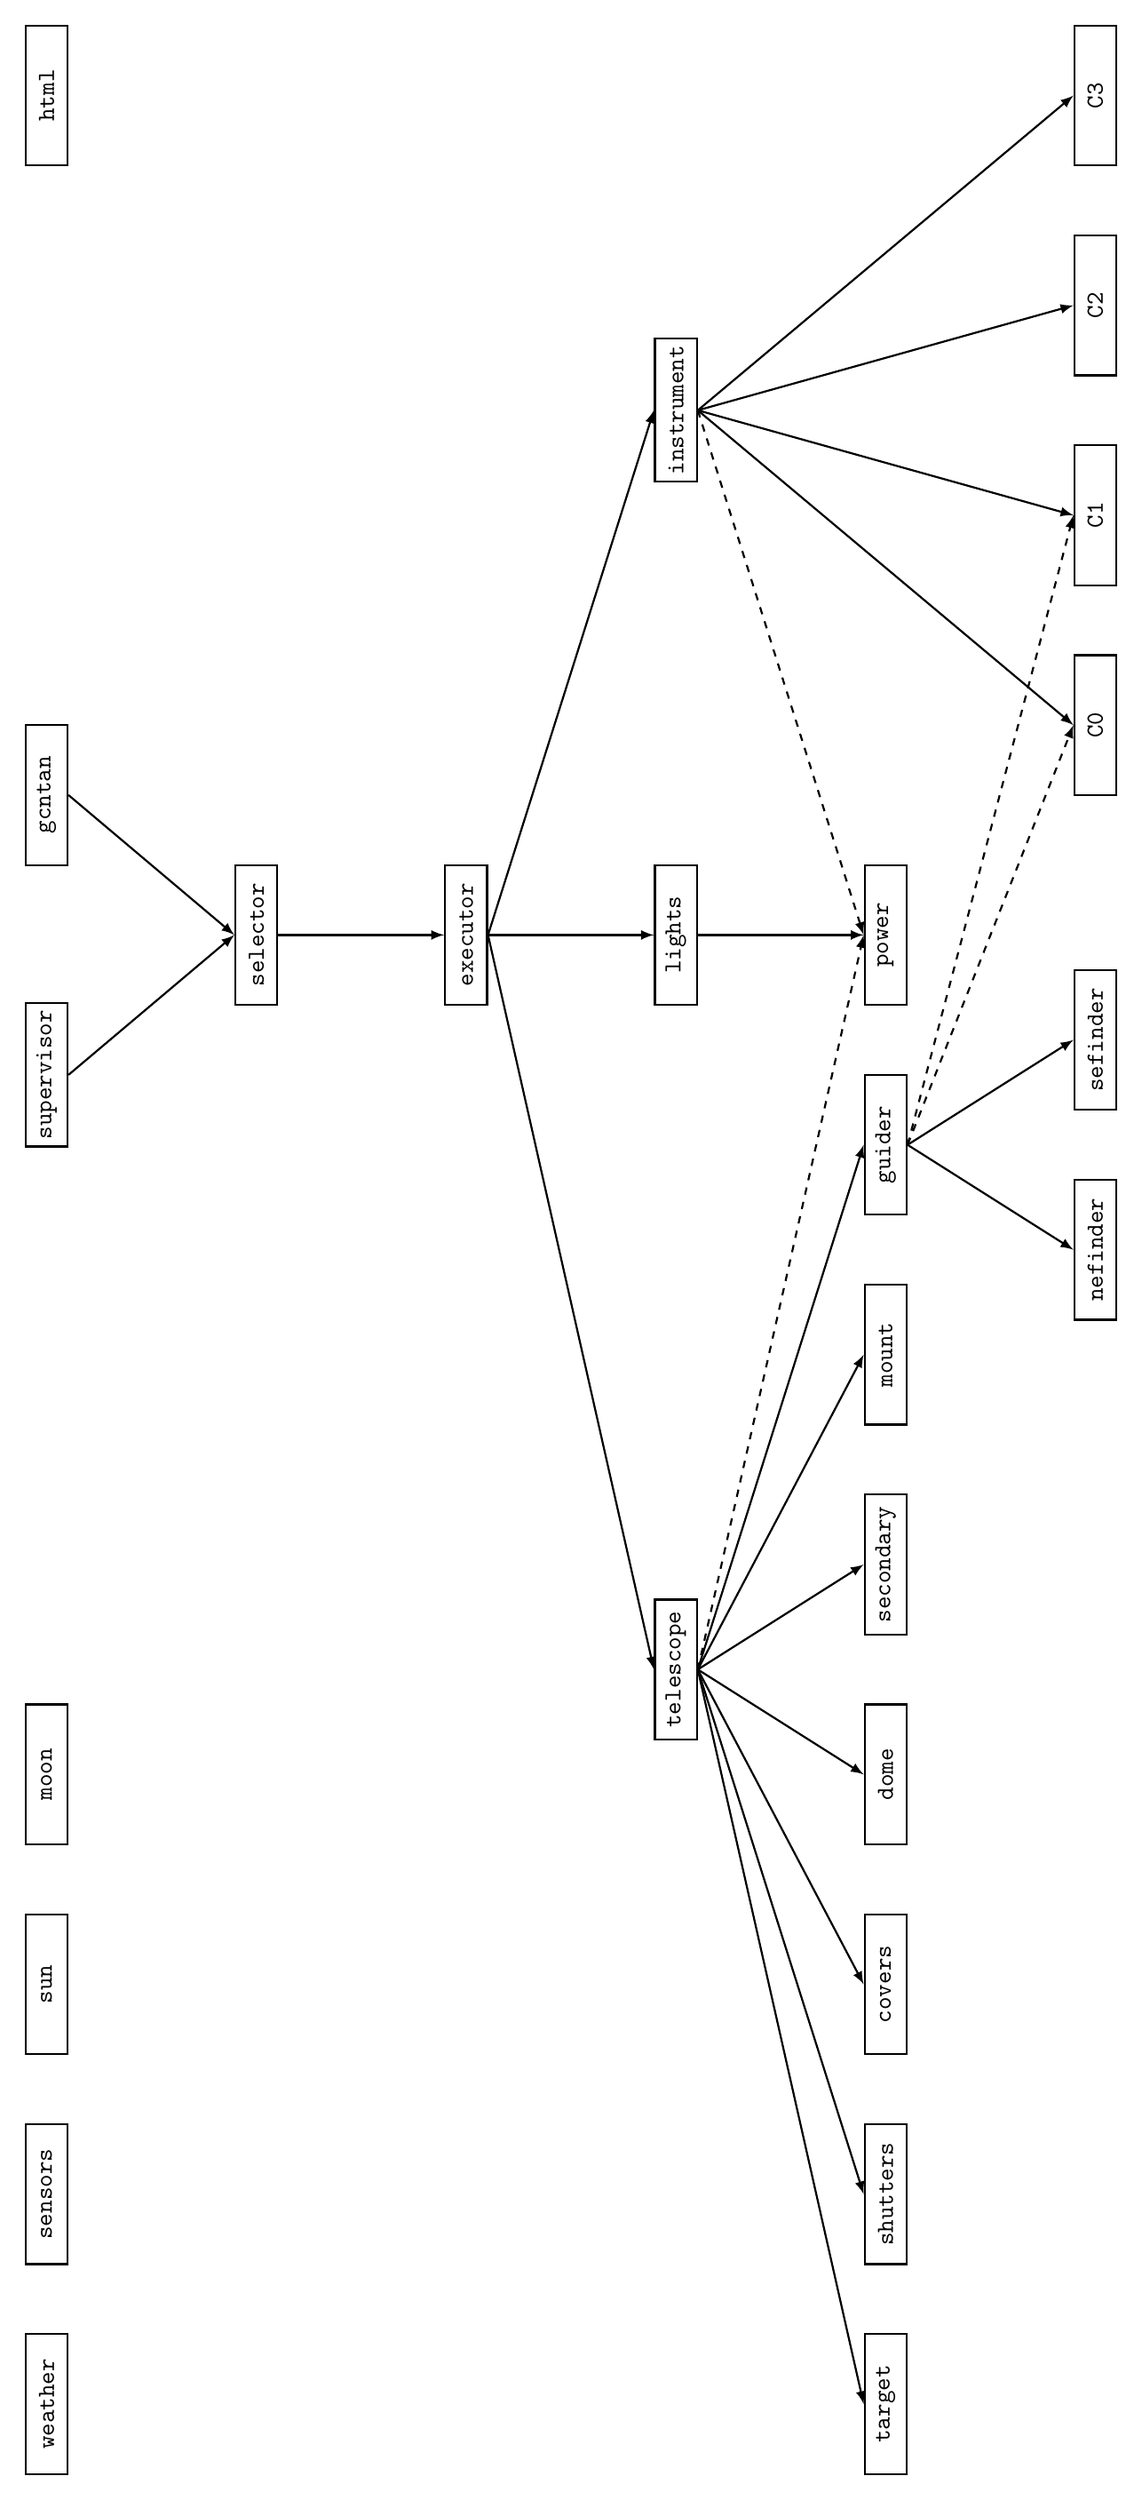
\begin{tikzpicture}[
 rotate=90,
 thick,
 >={latex},
 server/.style={
  inner sep=1mm,
  draw=black,
  rectangle,
  minimum width=2cm,
  minimum height=0.6cm,
  align=center,
  rotate=90,
 }
]

\node at (-21,-0) [server] (weather) {\server{weather}};
\node at (-18,-0) [server] (sensors) {\server{sensors}};
\node at (-15,-0) [server] (sun) {\server{sun}};
\node at (-12,-0) [server] (moon) {\server{moon}};

\node at (+12,-0) [server] (html) {\server{html}};

\node at (-2,-0) [server] (supervisor) {\server{supervisor}};
\node at (+2,-0) [server] (gcntan) {\server{gcntan}};
\node at (0,-3) [server] (selector) {\server{selector}};
\node at (0,-6) [server] (executor) {\server{executor}};

\draw[->] (supervisor.south) -- (selector.north);
\draw[->] (gcntan.south) -- (selector.north);
\draw[->] (selector.south) -- (executor.north);

\node at (-10.5,-9) [server] (telescope) {\server{telescope}};
\node at (-3,-12) [server] (guider) {\server{guider}};
\node at (-6,-12) [server] (mount) {\server{mount}};
\node at (-9,-12) [server] (secondary) {\server{secondary}};
\node at (-12,-12) [server] (dome) {\server{dome}};
\node at (-15,-12) [server] (covers) {\server{covers}};
\node at (-18,-12) [server] (shutters) {\server{shutters}};
\node at (-21,-12) [server] (target) {\server{target}};
\node at (-4.5,-15) [server] (nefinder) {\server{nefinder}};
\node at (-1.5,-15) [server] (sefinder) {\server{sefinder}};

\draw[->] (executor.south) -- (telescope.north);
\draw[->] (telescope.south) -- (guider.north);
\draw[->] (telescope.south) -- (mount.north);
\draw[->] (telescope.south) -- (secondary.north);
\draw[->] (telescope.south) -- (dome.north);
\draw[->] (telescope.south) -- (covers.north);
\draw[->] (telescope.south) -- (shutters.north);
\draw[->] (telescope.south) -- (target.north);
\draw[->] (guider.south) -- (nefinder.north);
\draw[->] (guider.south) -- (sefinder.north);

\node at (+7.5,-9) [server] (instrument) {\server{instrument}};
\node at (+3,-15) [server] (C0) {\server{C0}};
\node at (+6,-15) [server] (C1) {\server{C1}};
\node at (+9,-15) [server] (C2) {\server{C2}};
\node at (+12,-15) [server] (C3) {\server{C3}};

\draw[->] (executor.south) -- (instrument.north);
\draw[->] (instrument.south) -- (C0.north);
\draw[->] (instrument.south) -- (C1.north);
\draw[->] (instrument.south) -- (C2.north);
\draw[->] (instrument.south) -- (C3.north);
\draw[->,dashed] (guider.south) -- (C0.north);
\draw[->,dashed] (guider.south) -- (C1.north);

\node at (0,-9) [server] (lights) {\server{lights}};
\node at (0,-12) [server] (power) {\server{power}};

\draw[->] (executor.south) -- (lights.north);
\draw[->] (lights.south) -- (power.north);
\draw[->,dashed] (telescope.south) -- (power.north);
\draw[->,dashed] (instrument.south) -- (power.north);

\end{tikzpicture}
}
\end{center}
\caption{The server hierarchy in RATIR. The usual hierarchy is shown with solid arrows leading from the superior process to the inferior process. The temporary hierarchy around the use of \server{power} server by the \server{telescope} and \server{instrument} servers during opening and closing and the possible use of the \server{C0} or \server{C1} servers during guiding with the instrument.}
\label{figure:ratir-hierarchy}
\end{figure*}

The servers form a hierarchy in which an inferior server is only requested by its immediately superior server. Figure~\ref{figure:ratir-hierarchy} shows the server hierarchy for RATIR.

There is one general and two RATIR-specific exceptions to the hierarchy:

\begin{enumerate}
\item
The general is that any server can request information from any other server; that is the hierarchy restricts requests associated with \emph{actions} but not requests for \emph{information}.
\item
The first RATIR-specific exception is that the \server{power} server which controls the remote power switching hardware is used by various other superior servers (e.g., it controls the dome lights and the coolant pumps for the finder CCDs and the science CCDs). This could have been avoided by duplicating hardware and having an \server{power} server for each superior server, but in practice it has not been a problem, since the power is only switch during opening and closing and these actions are carefully sequenced.
\item
The second RATIR-specific exception is that the science CCDs controlled by the \server{C0} and \server{C1} servers are normally used for science observations and are controlled by the \server{instrument} superior server. However, we have implemented a special guiding mode in which we use one science CCD for guiding and the other for science observations, an when this mode is used one of the science CCD is controlled by the \server{guider} superior server. Again, use of this mode is carefully coordinated.
\end{enumerate}

These two RATIR-specific exceptions do not occur in the COATLI and DDOTI hierarchies, since there have a slightly different power control hardware and do not implement guiding. However, they show that sometimes multi-purpose hardware is most reasonably controlled by relaxing the strict server hierarchy.

We now briefly describe each of the servers in the RATIR hierarchy.

\begin{description}

\item[\server{supervisor}]~

The \server{supervisor} server is responsible for deciding when to open, when to close, and when to observe. The server has four possible states, which control its actions and which can be set by the observatory technical staff using the web interface:

\begin{itemize}
\item \variable{disabled}. In this state, the server does nothing. It is set to disabled in the morning, and so unless an action is taken to change this state the telescopes will not open.
\item \variable{enabled}. In this state, the server takes decisions to open, close, and observe according to the position of the Sun (obtained from the \server{sun} server) and the weather (obtained from the \server{weather} server). 
\item \variable{open}. In this state, the server takes decisions to open, close, and observe according to the position of the Sun (obtained from the \server{sun} server), but assumes the weather is fine. 
\item \variable{close}. In this state, the server closes regardless of the position of the Sun and the weather. 
\end{itemize}

The state is automatically is set to \variable{disabled} in the morning, and so unless an action is taken to change this state the telescopes will not open. Each afternoon, a member of the observatory technical staff inspects the telescope (physically or virtually using the webcams) and, if everything is fine, uses the web interface to the server state from \variable{disabled} to \variable{enabled}.

The weather station occasionally fails, especially after ice storms. The observatory technical can explicitly set the server state to \server{open} when the weather is benign. If the weather ceases to be benign, they set the server state to \server{close} to explicitly force it to close. This can also be used even when the weather station is working if they detect a reason to close that is not detected by the weather station (e.g., low clouds coming up the valleys to the north of the observatory) or for during night-time maintenance interventions.

\item[\server{gcntan}]~

The \server{gcntan} server listens on the GCN/TAN socket for alert packets. If one it received, it is decoded to give the type, identification, trigger time, position, and uncertainty. If the type is one that we have decided to follow (RATIR and COLIBRI respond to Swift and Fermi/LAT bursts, whereas DDOTI responds to these and also to Fermi/GBM bursts), the \server{gcntan} server requests the \server{selector} server to respond.

\item[\server{selector}]~

If the \server{selector} server is requested to \request{open} or \request{close}, it simply passes these requests down to the \server{executor} server. 

If the \server{selector} server is requested to \server{select}, it repeatedly selects a \emph{visit} from the queue and requests the executor to execute the visit. A \emph{visit} is our term for a unit of observations and is the term used for this in the context of the \emph{Hubble Space Telescope} and other NASA satellites, which for the RATIR team were our first contact with robotic observations in the 1990s. The equivalent term used by ESO is \emph{observing block}. In practical terms, a visit typically consists of a number of exposure at offsets about a single target coordinate position.

When the visit has finished executing, the selector either removes the visit from the queue or leaves it in the queue, according to a flag associated with each visit.

We have two queues. The higher priority queue contains visits for alert observations, which normally arrive via the \server{gcntan} server. The lower priority queue contains visits for science and calibration observations.

Each visit is associated with a set of constraints on hour angle, zenith distance, sky brightness, time since last focus, start time, and so on. The selector scans the alert queue in order. If it finds a visit whose constraints are all satisfied, it executes that visit. If not, it scans the normal visit queue in order. If it finds a visit whose constraints are all satisfied, it executes that visit. If not, it executes a special idle visit, which is typically to point at the zenith and take a dark.

Alert visits are typically left in the alert queue after being executed, so that an alert target is observed for as long as possible. During the day, the RATIR alert science team typically discusses the previous night’s alerts over Skype and decides to leave them in the queue or manually remove them. If the alert queue contains more than one visit, the order of the visits is rotated after each scan, so that for example, if the queue contains two alerts they are executed alternatively.

Science visits are typically removed from the normal queue after being executed. The order of visits is fixed. Thus, the selector makes no attempt at global optimization; our only recourse is to manually place visits in the queue in the desired order of priority. This is more or less manageable with RATIR, which typically only has a few non-alert science programs, but is an acknowledged weakness. Fortunately, it would be relatively easy to replace the scheduling algorithm with a more sophisticated one.

If the \server{selector} server is asked to respond to an alert, it firsts creates a new visit in the alert queue or updates an existing visit. (The visits are identified by source and trigger number.) This updating allows the coordinates to be refined, for example, when one or more Swift/XRT positions follow a Swift/BAT position.

Next, if this is a new alert (rather than just an update to the coordinates of an existing alert), if the \server{selector} server is observing (formally, if it is waiting for the \server{executor} server to finish executing a visit), and if the alert position is within the pointing limits, the \server{selector} server abandons the current visit. This forces a reselection, and the result of this will be to select the new alert.

Responding to an alert -- from receiving the GCN/TAN packet to beginning the slew -- typically takes only a fraction of a second.

\item[\server{weather}]~

The \server{weather} server is a passive server: it carries out no explicit actions and simply serves as an source of information.
The server communicates with the OAN/SPM central weather station and makes this information available other servers. In particular, it implements a status variable called \variable{maybeopen} which is true or false according to whether enclosures may be open by the rules agreed with the observatory on current and resent values of precipitation, wind speed, and humidity.

\item[\server{sun}]~

The \server{sun} server is a passive server: it carries out no explicit actions and simply serves as an source of information. The server simply determines the current position of the Sun and makes this information available to other servers.

\item[\server{moon}]~

The \server{moon} server is a passive server: it carries out no explicit actions and simply serves as an source of information. The server simply determines the current position of the Moon and makes this information available to other servers.

\item[\server{sensors}]~

The \server{sensors} server is a passive server: it carries out no explicit actions and simply serves as an source of information. The server polls the 1-wire temperature, humidity, light-level, and current sensors used to monitor the building and equipment and makes this information available to other servers.

\item[\server{executor}]~

The \server{executor} server coordinates the inferior \server{telescope}, \server{instrument}, and \server{lights} servers to open, close, and carry out visits.

If the \server{executor} server is requested to \request{open} or \request{opentocool} it switches on the lights, requests the instrument to open (which typically means cooling the detectors), requests the telescope to open, and then switches off the lights. The difference between \request{open} and \request{opentocool} is that the later only opens the enclosure partially and is used at the end of the day to allow the enclosure to cool before the start of twilight.

If the \server{executor} server is requested to \request{close}, it switches on the lights, requests the instrument to close (which typically means ceasing to cool the detectors), requests the telescope to close, and then leaves the lights on so that remote staff can verify that the enclosure has closed using the webcams. The executor automatically switches the lights off at sunrise.

If the \server{executor} server is requested to \request{execute} a visit, it runs the script associated with the visit. Running a script gives us the full power of a programming language; this is not normally needed for simple science visits, but it is useful for focusing and flat-field visits which need to adapt to the instrument’s measurements. The scripts for science visits are normally generated from a simple “Phase 2” description of the observations (a JSON file containing coordinates, constraints, and list of exposures and offsets) using a converter program. The scripts for calibration, focusing, and pointing correction are typically written by hand.

\item[\server{telescope}]~

The \server{executor} server coordinates the inferior servers associated with telescope hardware. Its main tasks are to open and close the dome shutters and telescope covers, to move to and track a target with the telescope, to track the telescope with the dome, to operate the guider.

\item[\server{target}]~

The \server{target} server determines the current position of the target (a fixed target with topocentric coordinates or a moving target with celestial coordinates and possibly a proper motion) and makes this information available to other servers.

\item[\server{mount}]~

The \server{mount} server controls the telescope mount. For equatorial telescope, this is the hour angle and declination drives.

\item[\server{secondary}]~

The \server{mount} server controls the secondary focus mechanism.

\item[\server{dome}]~

The \server{dome} server controls the dome rotation mechanism.

\item[\server{covers}]~

The \server{covers} server controls the telescope primary mirror covers.

\item[\server{shutters}]~

The \server{shutters} server controls the dome shutters.

\item[\server{guider}]~

The \server{guider} server has two main tasks.

First, it determines pointing corrections for the telescope using the two finder telescopes. 

Second, it uses the finders or one of the science CCDs to guide the telescope during exposures. This is necessary because the mechanics of the 1.5 meter telescope are so poor that it cannot track in open loop adequately for more than one minute without smearing the image.

\item[\server{nefinder}~\server{sefinder}]~

The server{nefinder} and \server{sefinder} servers control the finders.

RATIR has two finders, one on the north east side of the telescope and one on the south east side, because the dome is slightly undersized and there are positions where one finder or the other are occulted.

The finders are simple Celestron C8 telescope with FLI CCDs and focusers. We have removed the shutters from the CCDs to improve reliability. (The finders take of order 10,000 exposures per night and a shutter has a typical life of only about 500,000 cycles.) The finder field of view is about half a degree.

The finder servers are optimized for astrometry. After slewing to a field, the TCS takes images with both finders. It then runs SExtractor on the image to identify sources and astrometry.net on the source catalog to produce an astrometric solution. This takes about 1.5 seconds (typically 0.5 seconds for the exposure, 0.7 seconds to read the CCD, and 0.3 seconds to solve for the astrometry). The pointing information for the finder is transferred to the main telescope using a flexure model. Thus, two seconds after a slew has finished, the TCS has information to correct the pointing. This is the key to how we obtain reliable pointing with an old telescope.

Guiding is accomplished by simply repeatedly exposing and solving for the pointing. We are able to guide with a cadence of about 3 seconds. 

\item[\server{instrument}]~

The \server{instrument} server coordinates the instrument detectors, filter wheels, and focusers.

\item[\server{C0}~\server{C1}~\server{C2}~\server{C3}]~

RATIR has four “channels” called C0, C1, C2, and C3. Each channel has its own server which controls the detector (a CCD or H2RG), a filter wheel if present, and a focus stage if present.

Each server controls exposures, the detector cooler, the filter wheel, and the focuser. 

Additionally, each server has a very limited capability to analyze exposures in order to support real-time decisions by the instrument and executor servers. These are:
\begin{itemize}
\item Determining the signal level in the data section. This is used by the executor when taking flat fields to determine when to switch from one filter to another.
\item Determining the FWHM in the image. This is used by the executor when focusing. We have implemented three methods for determining the FWHM: estimated from the brightest non-saturated source detected by sextractor; estimate from the median of the non-saturated sources detected by sextractor; and estimated from fitting a Gaussian to the zero-shift peak in the autocorrelation of the image. The different methods ate useful in different circumstances. For example, autocorrelation is more robust on out-of-focus images and so is used for an initial rough focus position, but the sextractor methods are more precise when close to focus and are used for refining the rough focus position.
\item Determining the pointing by running the astrometry.net software. This is used at the start of the night to refine the relative pointing of the telescope and finders.
\end{itemize}

Each exposure is transferred to a central NAS as soon as it is completed, for analysis by the pipeline and eventual archiving.

\item[\server{html}]~

The \server{html} server polls the other servers for their state and writes the status and log fragments for the web interface.

\end{description}

\subsection{COATLI and DDOTI Servers}

The COATLI and DDOTI servers are identical to the RATIR servers down to the telescope and instrument servers.

COATLI and DDOTI have a custom telescope servers, mainly because they have folding enclosure and doesn’t have a dome, shutters, covers, or finders. All pointing correction is performed using the science instruments. Many of the hardware servers are different (for example, the mount server are for ASTELCO equatorial mounts rather than the legacy mount at the 1.5 meter telescope), but others are identical to RATIR (for example, the sensors server).

The TCS instrument server is generic and configurable, so the same code is used for RATIR with four detectors, COATLI with one detector, and DDOTI with two (soon to be six) detectors.

%Mechanism or sensor servers also interact appropriately with their associated hardware. 
%
%%In RATIR, all of the servers runs on two central computers and communication with remote hardware is either over the network or via USB extenders. In COATLI and DDOTI, 
%
%
%
%Each set of sensors is associated with a sensor server program. These servers essentially poll the state of the sensors and, when requested, supply it to clients.
%
%Each mechanism is associated with a mechanism server program. In addition to its other tasks, the server program polls the mechanism controller to determine the current state of the mechanism and, as a result of commands received, commands the mechanism controller. These mechanism controllers are isolated in the sense that one mechanism server never moves a mechanism other than the single one it controls (either directly or indirectly by issuing a request to another mechanism server), but some of them do request information from other servers. For example, the secondary controller applies an open-loop correction to the secondary position that depends on the temperature of the primary. Thus, the secondary server requests this information from the appropriate temperature-sensor server.
%
%The three most important celestial objects, the target, the sun, and the moon, are also associated with server programs. These provide clear points from which to obtain their positions. The sun and moon servers are quite similar to sensor servers, but instead of polling a sensor they calculate the position of the sun or moon. The target server is quite similar to a mechanism server, but when requested to move the target it simply notes the new coordinates rather than actually moving a mechanism.
%
%We have two higher-level servers that are the only servers that request other servers to move mechanisms or change internal state. The most pervasive of these is the master server, which coordinates all of the other servers in response to requests issued by the high-level TCS API. For example, when asked to move to a new target, it will: request the other servers to stop their current activity; then request the target server to note the coordinates of the new target; then ask the mount and dome to move to the new target; then request the secondary to perform an appropriate open-loop correction for flexure at the new position; then request the guider to determine the pointing error; then request the mount to correct for the pointing error; and finally indicate to the TCS client that the telescope is pointed at the new target. The other high-level server is the guider. When requested by the master server, it takes exposures with the two finder telescopes to determine the pointing and guiding errors.

\subsection{Human interface}

\begin{figure}
\begin{center}
\begin{tabular}{c}
\includegraphics[width=0.97\linewidth]{interface.png}
\end{tabular}
\end{center}
\caption{\label{figure:web-interface} 
The web page that implements the human interface, which is used mainly for testing, opening, and closing. The top row shows webcam images that allows the operator to check for obstructions and other impediments to operation. The second row are images from the science detectors. Below this is a line of links to pages that provide detailed information on each of the servers. In the middle left is a summary of the state of the mechanisms, sensors, and servers. In the middle right are controls. At the bottom is a log of messages from the TCS.}
\end{figure} 

%Despite being designed for an automated telescope, we felt that it was necessary to implement a more-or-less standard human interface to the TCS. This is used for testing and commissioning, to remotely open and close the telescope, and provides insight into the possibility of adapting the TCS for manual operation of the other telescopes of the OAN/SPM.

The human interface is implemented as a web page, and is shown in Figure~\ref{figure:web-interface}. It uses CGI programs to interact with the TCS and AJAX techniques to provide automatic updates. Implementing it as a web page gives us OS independence (it works with Firefox, Chrome, and Safari on Window, Mac OS X, iOS, Linux, and UNIX, but for reasons we have not been able to determine does not work with Internet Explorer on Windows) and allows us to use standard web authentication and access restriction mechanisms. The web interface is a standard TCS client; one CGI program obtains status information using the TCS API and another CGI program issues requests using the TCS API. Our experience with this interface is extremely positive; certainly, it feels as responsive as the previous Tk interfaces used at the telescope.

We also have a command-line interface which allows us to issue a request to any server by running an executable from the command line or from a script. This is very useful for testing and diagnosing problems.

\subsection{Implementation}

TCS is implemented almost entirely in Tcl, largely because when the project started, much of the observatory's software was already written in this language. If we were starting from scratch, we would probably have chosen Python, which is more widely known. 

On the other hand, this choice was not without practical benefits. Tcl has excellent support for asynchronous input and output, which is exactly what one needs in a telescope control system. Furthermore, Tcl 8.6 adds coroutines which allow one to express asynchronous programs more clearly than in the older event-driven style. We emphasize that we do not use the Tk graphics toolkit in the TCS; we simply use Tcl, without Tk, as a high-level programming language.

Our choice of a high-level language also simplified the interface between processes. Interaction between the client and the master server (i.e., the TCS client API) or between servers is by means of Tcl commands written to sockets. The receiving server simply reads a line of text and then executes it in an appropriate new slave interpreter. This eliminates the need write or adopt a parser for requests between servers. Similarly, we did not need to write or adopt a parser for configuration files; they are simply Tcl source files. These features are not unique to Tcl, but are a clear illustration of a practical advantage of using a dynamic high-level language over a static low-level language like C++. 

C/C++ is used for low-level interfaces to detectors and filter wheels (since these are typically exposed by C/C++ libraries) and for astrometric calculations (as a wrapper around SLALIB).

JavaScript is used for the web interface.

The code consists of about 10,000 lines of Tcl, 1000 lines of C/C++ (mainly for interfacing to detectors, filter wheels, and focusers and for writing FITS files), and 500 lines of JavaScript.

\section{Monitoring and Notification}

\subsection{Web Interface}

The TCS web interface provides real-time information on operations. It contains a summary page, which has an overview of the most important events of the night (opening, closing, and which visits have been executed), and more detailed global page which shows each low-level operation of all servers, and pages for each server which shows detailed state and each low-level operation for that server.

\subsection{Logs}

TCS logs all operations in a uniform manner to text log files. These files can be easily processed with tools like grep and awk to produce reports and look for problems.

\subsection{Plots}

TCS produce plots of variables such as sensor readings and weather. It produces plots over 4, 30, 120, and 500 days to allow one to detect trends.

\subsection{Nagios}

TCS uses the Nagios software to monitor the state of the observatory (e.g., power, environmental conditions, disk space, whether computers are up or not, whether server are running) and provide notification in case of unexpected problems. We have used this system  to be reliable and flexible.

We use email and the Pushover smart-phone application for notification. Pushover is free and is available for iOS and Android. It can be configured to react in different ways to different problems, for example, it can ring your phone continuously at any time of the day for serious problems or just give single silent notification for a less serious problem.

\section{Hardware}

In RATIR, COATLI, and DDOTI, TCS runs mainly on two 2010-era servers each with four cores and 8 GB of RAM. Even a typical 2018 entry-level server exceeds the capabilities of these servers.

In COATLI and DDOTI, the detector servers (including the real-time image analysis code) run on MinnowBoard SBCs with a dual-core Atom processor and 2 GB of RAM.

\section{Security}

We allow direct access to control aspects of TCS only from the mountain top, and enforce this at the firewall. Off-site staff gain access to the TCS using ssh to a host on the mountain and port-forwarding.

If desired, we could implement monitoring of the TCS (e.g., the information web pages but not the controls) with standard HTTP or HTTPS access mechanisms and make this available off-site. This would be a trivial modification.

Other security models are possible.

\section{Adapting TCS to COLIBRÍ}

What would it take to adapt TCS to COLIBRÍ?

\begin{itemize}
\item
Documentation. The current documentation for TCS is inadequate for a project beyond the initial RATIR group. 4 weeks, but this could be an on-going effort.
\item
JSON interface. As described in the DDRAGO control system document, we plan to move from using Tcl code for requests to server to the more neutral JSON-RPC. This would would be shared with DDRAGO. 1 week.
\item
Architecture. We would need to design an server and request architecture appropriate for COLIBRÍ, in collaboration with the other participants. Most of this is likely to follow RATIR, COATLI, and DDOTI, but there may be specific adaptions to CAGIRE and SVOM. 2 weeks.
\item
Implement the architecture using existing components. 1 week.
\item
PLC. COLIBRÍ uses a PLC for low-level control. We would need to interface TCS to this. 1 week.
\item
Alt-az Mount. TCS already controls ASTELCO \emph{equatorial} mounts using the OpenTCI interface, so the communication issues are largely solved. However, we would need to adapt it to an alt-az mount with a derotator. An initial effort would use the ASTELCO simple “POINTING” module, but this does not give full control of the pointing model and proper motions. A second iterations would program trajectories on each axis (as we already do with COATLI and DDOTI). 2 weeks for the initial effort. 2 weeks for the more advanced version.
\item
Interface to DDRAGO. 1 week.
\item
Interface to CAGIRE. 2 weeks.
\end{itemize}

I could have a simple version (JSON-RPC, architecture, existing components, and alt-az mount using the POINTING module) in 6 weeks: this could be used for initial testing at OHP. Then, during the tests at OHP we could integrate the PLC and DDRAGO.

We could run the COLIBRÍ software on two entry-level servers or a single mid-level server, although the entry-level servers would give better redundancy.

\section{Weaknesses}

The main weakness of TCS, in my opinion, is that the scheduler and proposal handing is extremely primitive.

The selector simply selects the first visit in the queue that satisfies all constraints. No attempt is made to optimize globally. The queue is typically ordered manually. This is not adequate for COLIBRÍ.

Proposal handling (communication with program PIs, receiving visits in Phase 2 format, conversion from Phase 2 format to visit scripts, placing the visits int he queue, monitoring the progress of programs) is entirely manual. Again, this is not adequate for COLIBRÍ.

In both of these areas, the proposals by Toulouse seem to be far superior to what we have in TCS. A wise option might be to integrate them into TCS (and test them  on the exiting UNAM telescopes prior to the deployment of COLIBRÍ).

\end{document}
